\chapter{Introduction}
\label{cha:Introduction}

\gls{SAT} is the problem of determining if there exists an interpretation that satisfies a given Boolean formula. Recently there has been substantial development in this area. Modern approach to SAT solving will use conflict-driven clause learning \footnote{\url{https://en.wikipedia.org/wiki/Conflict-driven_clause_learning}}, various heuristics and make use of better and better hardware. This rapid development in theory of solving SAT problems is followed by number of implementations. Picking best (fastest) implementation of SAT solver for given input problem is not trivial as solving algorithms are based on similar algorithm. Moreover SAT problem has NP complexity what encourages optimizing solvers to specific cases - that is if input formula has frequent pattern, it would be beneficial to optimize solver around that pattern. Input formulas can contain various theories \ref{pic:logicOverview} thus the need of benchmarks becomes apparent.

\begin{figure}[h]
\begin{centering}
  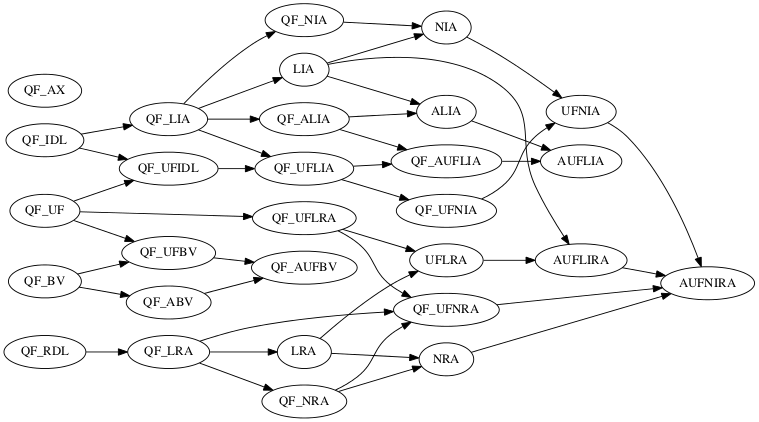
\includegraphics[width=0.7\textwidth]{images/smt_lib_logics.png}
  \caption{Overview of logic by SMT-LIB \url{http://smtlib.cs.uiowa.edu/logics.shtml}
    \tiny{
    QF - quantifier free formulas,
    A - or AX theory ArraysEx,
    BV - FixedSizeBitVectors,
    FP - (forthcoming) FloatingPoint theory,
    IA - theory Ints (Integer Arithmetic),
    RA - theory Reals (Real Arithmetic),
    IRA - theory Reals\_Ints (mixed Integer Real Arithmetic),
    IDL - Integer Difference Logic,
    RDL - Rational Difference Logic,
    L - linear,
    N - non-linear,
    UF - extension allowing free sort and function symbols
  }}
  \label{pic:logicOverview}
\end{centering}
\end{figure}

This thesis focuses on first order logic (with equolity) as tool for representing formulas. This is an attempt to create extensible, easy to use \gls{FOL} formula generator. Generator has this advantage over pregenerated dataset that it can precisely map encountered real-life problem into measurable, repeatable custom dataset. The goal is to hide implementation and display user simple interface with objects that correspond to mathematical definitions of elements of first order logic. Any arbitrary rule can be injected into generation to fulfill user specific needs. Those rules are meant to represent fragment or reality that user wants to represent in \gls{FOL}. Formulas generated in this way can be used as testing tool as randomness of formulas can be finely controlled. 

% https://en.wikipedia.org/wiki/Formal_system
% https://cs.lmu.edu/~ray/notes/formalsystems/

\chapter{Logical systems}
% https://en.wikipedia.org/wiki/Mathematical_logic#Formal_logical_systems
% https://en.wikipedia.org/wiki/Formal_system#Logical_system
% https://en.wikipedia.org/wiki/Formal_system
% https://cs.lmu.edu/~ray/notes/formalsystems/

Formulas must be presented in some kind of formal system. A formal system consists of a language over some alphabet of symbols together with (axioms and) inference rules that distinguish some of the strings in the language as theorems. These rules used to carry out the inference of theorems from axioms are known as the logical calculus of the formal system. A formal system may represent a well-defined system of abstract thought. A logical systemis a formal system together with its semantics. Some recognizable logical formal systems are:

\begin{itemize}
  \item propositional logic 
  \item first order logic (FOL)
  \item higher order logic (HOL)
  \item temporal logic 
\end{itemize}

The majority of formulas are probably going to be represented in propositional calculus because of simplicity of such notation. Propositional logic deals with variables which are connected with logical connectives. Variable can be true or false. Formula in propositional logic is easy to parse but may lack clarity and may be quite long when compared to different formal logical systems. For more complex problem it may be easier to encode problem in more expressive language and the next natural step would be first order logic. \gls{FOL} has tools for expressing relation and still is easy enough to implement and reason in automated way. 

\section{First Order Logic}

The main element of propositional calculus is variable. First order logic (also known as predicates logic, first-order predicate calculus) extends propositional logic by adding predicates, functors and quantifiers and non-logical objects. Definitions of FOL elements are contained below.

\textbf{Term}
is variable, constant or result of functor.

\textbf{Atom}
is logical statement, that can not be further divided. Atom consists of predicate, or in case of atom with equality it consists of terms.

\textbf{Literal}
is atom or its negation.

% http://mathworld.wolfram.com/First-OrderLogic.html
\textbf{Variable}
unlike propositional logic, variables in \gls{FOL} can stand for a relation (between terms) but which has not been specifically assigned any particular relation.
Usually starts with capital letter. If variables is used in quantifier it is called bound variable, otherwise it is called free variable.

\textbf{Singleton variable}
is used only once in clause

\textbf{Clause}
is disjunction of literals

\textbf{Unit clause}
is clause with only one literal

\textbf{Horn clause}
is clause, which contains at least one positive literal

\textbf{Predicates}
is logical operator, which return true or false. predicates operates on specific number of terms. This number is constant and called predicate \textbf{arity}. Usually noted as $predicate\_name/arity$, eg. $p/1$. Name of predicate is usually lowercase $p, q, r $

\textbf{Functor}
is logical operator, that returns term. Functor has constant arity. Usually noted as $functor\_name/arity$, eg. $f/1$. Name of functor  is usually lowercase $f, g, h$

\textbf{Constant functor}
is functor with arity 0.

% https://en.wikipedia.org/wiki/Quantifier_(logic)
\textbf{Quantifier}
specifies the quantity of specimens in the universe that satisfy an open formula (formula with at least one free variable). A formula beginning with a quantifier is called a quantified formula.

\textbf{Existential quantifier}
is equivalent to a logical disjunction of propositions, this is, at least one proposition must be true.

\textbf{Universal quantifier}
is equivalent to a logical conjunction of propositions, this is, all propositions must be true.

The following \gls{FOL} example contains 1 existential quantifier, 2 variables $W$, $Z$, 1 predicate $p/2$, 2 constant functors $a/0$, $b/0$.
\begin{equation} \label{eg:FOL_1}
  \exists_{W,Z} p(W,Z) | p(a, b)
\end{equation}

\section{Normal forms}

Representing logic formula in one of normal forms sometimes can enable new or shorter reasoning not available otherwise. One of normal forms mentioned in this thesis is \textbf{conjunctive normal form (CNF)}. It is a conjunction of one or more clauses, where a clause is a disjunction of literals. Other example of normal form is disjunctive normal form (DNF) where formula is disjunction of conjunctions.

\section{Formats used for representing formulas}

There are many formats that allow representing logic, for example:

\begin{itemize}
  \item DIMACS - one of more popular formats for propositional logic 
  \item \gls{LADR} - input format for Prover9 \footnote{Prover9 is an automated theorem prover for first-order and equational logic \url{https://www.cs.unm.edu/~mccune/mace4/}}
  \item SMT-LIB - standard for encoding SMT problems, used for example by Z3 solver
  \item \gls{TPTP} 
\end{itemize}

Many provers implement its own language for representing logic formulas like prover9 what creates technical problems of compability between solvers. In this thesis a standard called \gls{TPTP} will be used to represent first order logic formulas.

\subsection{Thousands of Problems for Theorem Provers}

TPTP \cite{Sut17} - Thousands of Problems for Theorem Provers - is both problem library used for testing \gls{ATP} systems and standard describing syntax for those tests. Next to TPTP library there is \gls{TSTP} - library of solutions produced by various solvers. Problems are classified into different domains: LCL - Logic Calculi, COL - Combinatory Logic and more.

TPTP defines syntax for several logic systems: \gls{TPI}, \gls{THF}, \gls{TFF}, \gls{FOF}, \gls{CNF} but in this thesis only \gls{FOF} and \gls{CNF} will be used.

\subsubsection{First order logic in TPTP syntax}

Full description (technical document) for TPTP syntax can be found at \url{http://www.tptp.org/TPTP/TR/TPTPTR.shtml}

\begin{itemize}
  \item Variables start with upper case letters, atoms and terms are written in prefix notation, uninterpreted predicates and functors either start with lower case and contain alphanumerics and underscore, or are in 'single quotes'.

  \item Each logical formula is wrapped in an annotated formula structure of the form \mintinline{text}{fof(name,role,formula,source,[useful_info])} or \mintinline{text}{cnf(name,role,formula,source,[useful_info])}

    \begin{itemize}
      \item \mintinline{text}{name} is only for documenting purposes
      \item \mintinline{text}{role} gives the user semantics of the formula, in context of SAT problem it will be usually \mintinline{text}{axiom}, but can also for example \mintinline{text}{hypothesis} or \mintinline{text}{definition}. They are accepted, without proof, as a basis for proving conjectures. In CNF problems the axiom-like formulae are accepted as part of the set whose satisfiability has to be established. A problem is solved only when all formulas with role \mintinline{text}{conjecture} are proven. TPTP problems never contain more than one conjecture. \mintinline{text}{negated_conjectures} are formed from negation of a \mintinline{text}{conjecture}, typically in FOF to CNF conversion.
      \item \mintinline{text}{formula} is logical formula
      \item the \mintinline{text}{source} field is used to record where the annotated formula came from, and is most commonly a file record or an inference record
      \item the \mintinline{text}{useful_info} field of an annotated formula is optional, and if it is not used then the \mintinline{text}{source} field becomes optional
    \end{itemize}

  \item The language also supports interpreted predicates and functors. These come in two varieties: 
    \begin{itemize}
      \item defined predicates and functors, whose interpretation is specified by the TPTP language like \mintinline{text}{$true} and \mintinline{text}{$false}, \mintinline{text}{=} and \mintinline{text}{!=} and arithmetic predicates
      \item system predicates and functors, whose interpretation is \gls{ATP} system specific, like \mintinline{text}{$o} - the Boolean type, \mintinline{text}{$i} - the type of individuals, \mintinline{text}{$real} - the type of reals, \mintinline{text}{$rat} - the type of rational, and \mintinline{text}{$int} - the type of integers.
    \end{itemize}

  \item The universal quantifier is \mintinline{text}{!}, the existential quantifier is \mintinline{text}{?}, and the lambda binder is \mintinline{text}{^}. Quantified formulae are written in the form \mintinline{text}{Quantifier [Variables] :  Formula}

  \item The binary connectives are infix \mintinline{text}{|} for disjunction, infix \mintinline{text}{&} for conjunction, infix \mintinline{text}{<=>} for equivalence, infix \mintinline{text}{=>} for implication, infix \mintinline{text}{<=} for reverse implication, infix \mintinline{text}{<~>} for non-equivalence (XOR), infix \mintinline{text}{~|} for negated disjunction (NOR), infix	\mintinline{text}{~&} for negated conjunction (NAND), infix \mintinline{text}{@} for application. The only unary connective is prefix \mintinline{text}{~} for negation

\subsubsection{Additional tools in TPTP library}
\label{sub:AdditionalToolsInTPTPLibrary}

TPTP ships with \gls{TPTP4X} (written in c), \gls{TPTP2X} (written in prolog) utilities, which are used for reformatting, transforming, and generating TPTP problem files. Example of functionalities:

\begin{itemize}
  \item converting \gls{FOF} to \gls{CNF} (eg. with otter \cite{McC-Otter-URL}, bundy \cite{Bun83} algorithm, details in \cite{SM96})
  \item converting TPTP to syntax required by prover9, dimacs, otter, dfg and more
  \item optimization \gls{FOF}, \gls{CNF} with different algorithms
  \item change order of \gls{CNF}
\end{itemize}

\subsubsection{Examples of FOL and CNF in TPTP syntax}

For comparison examples of \gls{FOL} formulas are also shown in CNF. 

\begin{listing}[H]
  \caption{TPTP FOL formula with existential quantifier, translated to CNF}
\begin{tptpcode}
fof(simple_exists, axiom,
 ? [W,Z] : p(W, Z) | p(a, b)
  ).
% equivalent in CNF, converted with TPTP2X, otter algorithm
cnf(simple_exists_1,axiom,
    ( p(sk1,sk2) | p(a,b) )).
\end{tptpcode}
\end{listing}

\begin{listing}[H]
  \caption{TPTP FOL formula with universal quantifier, translated to CNF}
\begin{tptpcode}
fof(simple_for_all, axiom,
 ! [W,Z] : p(W, Z) | p(a, b)
  ).
% equivalent in CNF, converted with TPTP2X, otter algorithm
cnf(simple_for_all_1,axiom,
    ( p(A,B) | p(a,b) )).
\end{tptpcode}
\end{listing}

\begin{listing}[H]
  \caption{TPTP FOL formula, translated to CNF}
\begin{tptpcode}
% for every X, Y operation lesseq is the same as less or equal
fof(this_is_obvious, axiom,
  ! [X,Y] : ( $lesseq(X,Y) <=> ( $less(X,Y) | X = Y ) )
  ).
% equivalent in CNF, converted with TPTP2X, otter algorithm
cnf(this_is_obvious_1,axiom,
    ( ~ $lesseq(A,B) | $less(A,B) | A = B )).

cnf(this_is_obvious_2,axiom,
    ( ~ $less(A,B) | $lesseq(A,B) )).

cnf(this_is_obvious_3,axiom,
    ( A != B | $lesseq(A,B) )).
\end{tptpcode}
\end{listing}

